\documentclass[border=4pt,12pt]{standalone}
% House style for redrawn exam diagrams (diagram-v4: 0.4pt lines, filled -latex arrows, fine dashes; stipple and hatching drawn as real dots/lines (no PDF/SVG patterns, so they render in every browser and at any scale); transparent background). Every figure \input's this.
\usepackage{amsmath,amssymb}
\usepackage{txfonts}
\usepackage{pdfrender,xcolor}
% \halo{text}: label on shading. The shading stops just around each letter's outline (a thin knock-out that follows the
% glyphs, like the papers' typesetting), never a box. Owner: "I don't want a box around the text".
\newcommand{\halo}[1]{\leavevmode\rlap{\pdfrender{TextRenderingMode=2,LineWidth=2.2pt,LineJoinStyle=1,StrokeColor=white,FillColor=white}#1}#1}
\usepackage{tikz,pgfplots}
\pgfplotsset{compat=1.18}
\usetikzlibrary{arrows.meta,calc,angles,quotes,patterns,patterns.meta,intersections,positioning,decorations.markings,shapes.geometric}
% Stipple and hatching are drawn as actual dots / lines clipped to the region (path picture), NOT as pattern fills:
% SVG <pattern> fills vanish or blur when browsers scale the image, so the owner could not see the shading.
% Each dot is a 0.72pt square (keeps SVGs small; reads as a dot at print size). Dots sit on one global staggered grid, so neighbouring regions line up.
\makeatletter
\newdimen\ex@x \newdimen\ex@y \newdimen\ex@xa \newdimen\ex@ya \newdimen\ex@xb \newdimen\ex@yb \newcount\ex@row
\def\exam@stipplecolor{black!75}\def\exam@dotr{0.42pt}\def\exam@dotgap{2.5}
\def\ex@rowdots{\ifdim\ex@x<\ex@xb \pgfpathrectangle{\pgfqpoint{\dimexpr\ex@x-0.36pt\relax}{\dimexpr\ex@y-0.36pt\relax}}{\pgfqpoint{0.72pt}{0.72pt}}\advance\ex@x by \exam@dotgap pt\relax\expandafter\ex@rowdots\fi}
\def\exam@stipple{%
  \pgftransformreset% dots are sized in real points even inside scaled pictures
  \pgfpointanchor{path picture bounding box}{south west}\ex@xa=\pgf@x \ex@ya=\pgf@y
  \pgfpointanchor{path picture bounding box}{north east}\ex@xb=\pgf@x \ex@yb=\pgf@y
  \pgfsetfillcolor{\exam@stipplecolor}\pgfmathsetmacro\ex@h{\exam@dotgap/2}%
  \pgfmathtruncatemacro\ex@r{floor(\ex@ya/\ex@h)-1}\ex@row=\ex@r\relax
  \ex@y=\ex@r\dimexpr\ex@h pt\relax
  \loop\ifdim\ex@y<\ex@yb
    \pgfmathtruncatemacro\ex@c{floor(\ex@xa/\exam@dotgap)-1}\ex@x=\ex@c\dimexpr\exam@dotgap pt\relax
    \ifodd\ex@row \advance\ex@x by \ex@h pt\fi
    \ex@rowdots
    \advance\ex@y by \ex@h pt \advance\ex@row by 1
    \ifnum\numexpr\ex@row-(\ex@row/4)*4\relax=0 \pgfusepath{fill}\fi% flush every 4 rows: bounded TeX memory, few clip copies in the SVG
  \repeat\pgfusepath{fill}}
\newdimen\ex@d
\def\exam@hatch#1{% #1 = 1 for /, -1 for \ ; lines 45 degrees, 3pt apart
  \pgftransformreset
  \pgfpointanchor{path picture bounding box}{south west}\ex@xa=\pgf@x \ex@ya=\pgf@y
  \pgfpointanchor{path picture bounding box}{north east}\ex@xb=\pgf@x \ex@yb=\pgf@y
  \ex@d=\dimexpr\ex@yb-\ex@ya\relax \ex@x=\dimexpr\ex@xa-\ex@d\relax
  \loop\ifdim\ex@x<\ex@xb
    \ifnum#1>0 \pgfpathmoveto{\pgfqpoint{\ex@x}{\ex@ya}}\pgfpathlineto{\pgfqpoint{\dimexpr\ex@x+\ex@d\relax}{\ex@yb}}%
    \else \pgfpathmoveto{\pgfqpoint{\ex@x}{\ex@yb}}\pgfpathlineto{\pgfqpoint{\dimexpr\ex@x+\ex@d\relax}{\ex@ya}}\fi
    \advance\ex@x by 4.24pt
  \repeat
  \pgfsetlinewidth{0.4pt}\pgfsetstrokecolor{black}\pgfusepath{stroke}}
\def\examstipple{\exam@stipple}\def\examhatch{\exam@hatch}\def\examsetstipplecolor#1{\def\exam@stipplecolor{#1}}\def\examsetdotgap#1{\def\exam@dotgap{#1}}
\makeatother
% (legacy pattern kept for old files)
% staggered stipple like the NESA papers' dotted shading
\pgfdeclarepatternformonly{exam stipple}{\pgfpointorigin}{\pgfqpoint{2.2pt}{2.2pt}}{\pgfqpoint{2.2pt}{2.2pt}}{%
  \pgfpathcircle{\pgfqpoint{0.55pt}{0.55pt}}{0.42pt}\pgfpathcircle{\pgfqpoint{1.65pt}{1.65pt}}{0.42pt}\pgfusepath{fill}}
\tikzset{
  every picture/.style={line width=0.6pt, >={Latex[length=2mm,width=1.3mm]}},
  curve/.style={line width=0.6pt},
  open arrow/.style={-{Latex[length=2mm,width=1.3mm]}},  % owner: filled -latex heads everywhere, no open chevrons
  aux/.style={dash pattern=on 2pt off 1.5pt, line width=0.6pt},
  shade/.code={\def\exA{#1}\def\exB{none}\ifx\exA\exB\else\pgfkeysalso{fill=black!18}\fi},
  shade/.default=on,
  shade dots/.style={fill=none, path picture={\examstipple}},
  stipple color/.code={\examsetstipplecolor{#1}},
  stipple gap/.code={\examsetdotgap{#1}},
  shade dense dots/.style={fill=none, stipple gap=1.6, path picture={\examstipple}},
  shade hatch/.style={fill=none, path picture={\examhatch{1}}},
  shade hatch reverse/.style={fill=none, path picture={\examhatch{-1}}},
  shade solid/.style={fill=black},
  pt/.style={circle, fill, inner sep=1.1pt},
  open pt/.style={circle, draw, fill=white, inner sep=1.1pt},
}
\pgfplotsset{
  exam axes/.style={axis lines=middle, axis line style={->}, xlabel={$x$}, ylabel={$y$},
    xlabel style={anchor=west}, ylabel style={anchor=south}, tick label style={font=\small},
    every axis plot/.append style={line width=0.6pt, black}, samples=200, clip=false,
    enlargelimits=false, axis on top},
}

\begin{document}
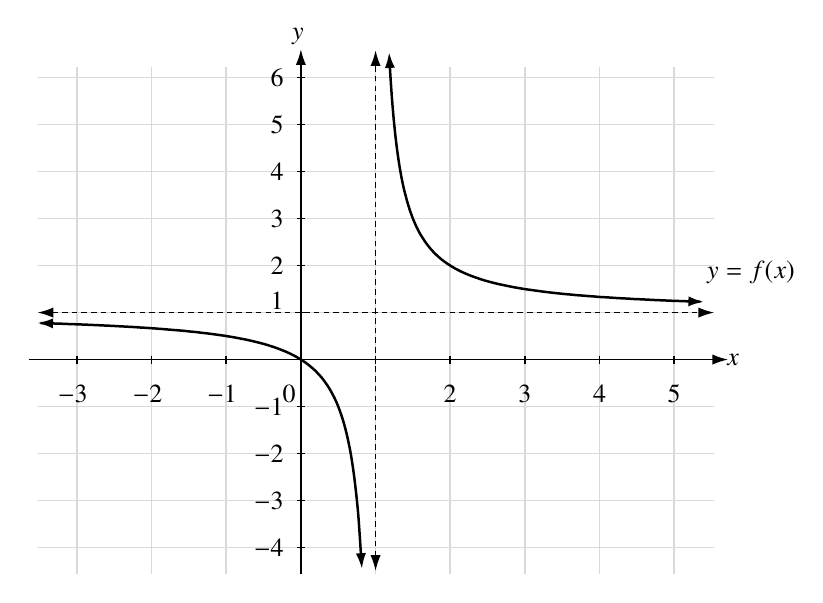
\begin{tikzpicture}[x=0.0127cm,y=-0.0127cm,font=\fontsize{9.4}{11.28}\selectfont]
\begin{scope}\clip (9,55) rectangle (686,562);
\draw[black!15] (48.4,0)--(48.4,562);
\draw[black!15] (123.1,0)--(123.1,562);
\draw[black!15] (197.8,0)--(197.8,562);
\draw[black!15] (347.2,0)--(347.2,562);
\draw[black!15] (421.9,0)--(421.9,562);
\draw[black!15] (496.6,0)--(496.6,562);
\draw[black!15] (571.3,0)--(571.3,562);
\draw[black!15] (646.0,0)--(646.0,562);
\draw[black!15] (720.7,0)--(720.7,562);
\draw[black!15] (0,535.5)--(770,535.5);
\draw[black!15] (0,488.5)--(770,488.5);
\draw[black!15] (0,441.5)--(770,441.5);
\draw[black!15] (0,394.5)--(770,394.5);
\draw[black!15] (0,300.5)--(770,300.5);
\draw[black!15] (0,253.5)--(770,253.5);
\draw[black!15] (0,206.5)--(770,206.5);
\draw[black!15] (0,159.5)--(770,159.5);
\draw[black!15] (0,112.5)--(770,112.5);
\draw[black!15] (0,65.5)--(770,65.5);
\draw[black!15] (0,18.5)--(770,18.5);
\end{scope}
\draw[->] (0,347.5)--(700,347.5); \draw[->] (272.5,562)--(272.5,37);
\draw (48.4,343.5)--(48.4,351.5); \draw (123.1,343.5)--(123.1,351.5); \draw (197.8,343.5)--(197.8,351.5); \draw (347.2,343.5)--(347.2,351.5); \draw (421.9,343.5)--(421.9,351.5); \draw (496.6,343.5)--(496.6,351.5); \draw (571.3,343.5)--(571.3,351.5); \draw (646.0,343.5)--(646.0,351.5);
\draw (268.5,535.5)--(276.5,535.5); \draw (268.5,488.5)--(276.5,488.5); \draw (268.5,441.5)--(276.5,441.5); \draw (268.5,394.5)--(276.5,394.5); \draw (268.5,300.5)--(276.5,300.5); \draw (268.5,253.5)--(276.5,253.5); \draw (268.5,206.5)--(276.5,206.5); \draw (268.5,159.5)--(276.5,159.5); \draw (268.5,112.5)--(276.5,112.5); \draw (268.5,65.5)--(276.5,65.5);
\draw[aux,<->] (347.2,559)--(347.2,38); \draw[aux,<->] (9,300.5)--(686,300.5);
\draw[<->, line width=0.9pt] plot[smooth] coordinates {(8.8,310.9) (12.5,311.0) (16.1,311.1) (19.8,311.2) (23.4,311.3) (27.1,311.5) (30.7,311.6) (34.3,311.7) (38.0,311.9) (41.6,312.0) (45.3,312.1) (48.9,312.3) (52.6,312.4) (56.2,312.6) (59.9,312.7) (63.5,312.9) (67.2,313.0) (70.8,313.2) (74.5,313.4) (78.1,313.5) (81.8,313.7) (85.4,313.9) (89.1,314.1) (92.7,314.3) (96.4,314.5) (100.0,314.7) (103.7,314.9) (107.3,315.1) (111.0,315.4) (114.6,315.6) (118.3,315.8) (121.9,316.1) (125.6,316.3) (129.2,316.6) (132.9,316.9) (136.5,317.2) (140.1,317.5) (143.8,317.8) (147.4,318.1) (151.1,318.4) (154.7,318.7) (158.4,319.1) (162.0,319.5) (165.7,319.8) (169.3,320.2) (173.0,320.7) (176.6,321.1) (180.3,321.5) (183.9,322.0) (187.6,322.5) (191.2,323.0) (194.9,323.5) (198.5,324.1) (202.2,324.7) (205.8,325.3) (209.5,326.0) (213.1,326.7) (216.8,327.4) (220.4,328.2) (224.1,329.0) (227.7,329.9) (231.4,330.8) (235.0,331.8) (238.7,332.8) (242.3,334.0) (246.0,335.2) (249.6,336.5) (253.2,337.9) (256.9,339.4) (260.5,341.0) (264.2,342.8) (267.8,344.7) (271.5,346.9) (275.1,349.2) (278.8,351.8) (282.4,354.7) (286.1,357.9) (289.7,361.6) (293.4,365.7) (297.0,370.5) (300.7,376.0) (304.3,382.4) (308.0,390.0) (311.6,399.2) (315.3,410.5) (318.9,424.6) (322.6,443.0) (326.2,467.8) (329.9,503.0) (333.5,557.0)};
\draw[<->, line width=0.9pt] plot[smooth] coordinates {(360.7,40.0) (361.5,54.7) (362.3,67.8) (363.1,79.5) (363.9,90.2) (364.7,99.8) (365.5,108.6) (366.3,116.7) (367.1,124.1) (367.9,131.0) (368.7,137.3) (369.5,143.2) (370.3,148.7) (371.1,153.8) (371.9,158.5) (372.7,163.0) (373.5,167.2) (374.3,171.1) (375.1,174.9) (375.9,178.4) (376.8,181.7) (377.6,184.8) (378.4,187.8) (379.2,190.7) (380.0,193.3) (380.8,195.9) (381.6,198.4) (382.4,200.7) (383.2,202.9) (384.0,205.1) (384.8,207.1) (385.6,209.0) (386.4,210.9) (387.2,212.7) (388.0,214.5) (388.8,216.1) (389.6,217.7) (390.4,219.3) (391.2,220.7) (392.0,222.2) (397.8,231.1) (403.6,238.3) (409.4,244.1) (415.2,248.9) (421.0,252.9) (426.8,256.4) (432.6,259.4) (438.4,262.0) (444.2,264.3) (450.0,266.3) (455.7,268.2) (461.5,269.8) (467.3,271.3) (473.1,272.6) (478.9,273.8) (484.7,275.0) (490.5,276.0) (496.3,277.0) (502.1,277.8) (507.9,278.6) (513.7,279.4) (519.5,280.1) (525.3,280.8) (531.1,281.4) (536.8,282.0) (542.6,282.5) (548.4,283.1) (554.2,283.5) (560.0,284.0) (565.8,284.4) (571.6,284.9) (577.4,285.2) (583.2,285.6) (589.0,286.0) (594.8,286.3) (600.6,286.6) (606.4,287.0) (612.2,287.2) (617.9,287.5) (623.7,287.8) (629.5,288.1) (635.3,288.3) (641.1,288.6) (646.9,288.8) (652.7,289.0) (658.5,289.2) (664.3,289.4) (670.1,289.6) (675.9,289.8)};
\node[anchor=base,inner sep=0] at (44.4,390) {$-3$}; \node[anchor=base,inner sep=0] at (119.1,390) {$-2$}; \node[anchor=base,inner sep=0] at (193.8,390) {$-1$}; \node[anchor=base,inner sep=0] at (421.9,390) {$2$}; \node[anchor=base,inner sep=0] at (496.6,390) {$3$}; \node[anchor=base,inner sep=0] at (571.3,390) {$4$}; \node[anchor=base,inner sep=0] at (646.0,390) {$5$};
\node[anchor=base east,inner sep=0] at (268,390) {$0$};
\node[anchor=east,inner sep=0] at (256,535.5) {$-4$}; \node[anchor=east,inner sep=0] at (256,488.5) {$-3$}; \node[anchor=east,inner sep=0] at (256,441.5) {$-2$}; \node[anchor=east,inner sep=0] at (256,394.5) {$-1$}; \node[anchor=east,inner sep=0] at (256,253.5) {$2$}; \node[anchor=east,inner sep=0] at (256,206.5) {$3$}; \node[anchor=east,inner sep=0] at (256,159.5) {$4$}; \node[anchor=east,inner sep=0] at (256,112.5) {$5$}; \node[anchor=east,inner sep=0] at (256,65.5) {$6$};
\node[anchor=south east,inner sep=0] at (256,298.5) {$1$};
\node[anchor=base west,inner sep=0] at (263,27) {$y$};
\node[anchor=base west,inner sep=0] at (697,353) {$x$};
\node[anchor=base west,inner sep=0] at (678,266) {$y=f(x)$};\end{tikzpicture}
\end{document}
